\documentclass[tikz, border=10pt]{standalone}
\usetikzlibrary{shapes.geometric, arrows.meta, positioning, calc}

\begin{document}
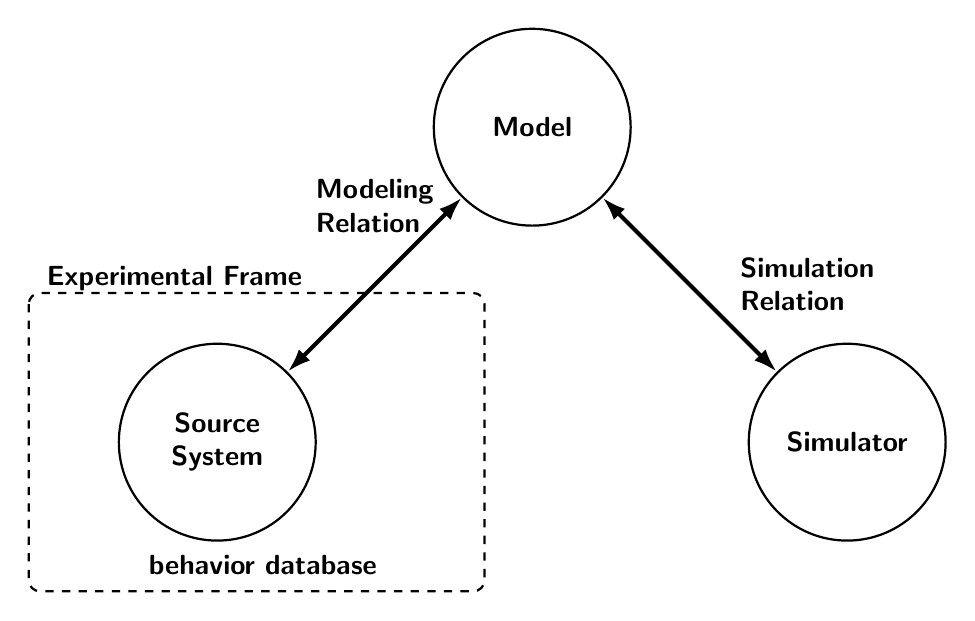
\begin{tikzpicture}[
    font=\sffamily,
    thick,
    main node/.style={
        circle, 
        draw=black, 
        thick, 
        minimum size=2.5cm, 
        align=center, 
        font=\sffamily\bfseries
    },
    relation label/.style={
        font=\sffamily\bfseries, 
        align=left
    }
]

    \node[main node] (source) at (0,0) {Source\\System};
    \node[main node] (model) at (4, 4) {Model};
    \node[main node] (sim) at (8, 0) {Simulator};

    % --- Experimental Frame ---
    \draw[thick, dashed, rounded corners] 
        ($(source.north west) + (-1.5, 1.0)$) rectangle 
        ($(source.south east) + (2.5, -1.0)$);

    \node[anchor=south west] at ($(source.north west) + (-1.4, 0.9)$) {\textbf{Experimental Frame}};
    \node[anchor=west] at ($(source.south) + (-1, -0.3)$) {\textbf{behavior database}};

    \draw[{Latex[length=3mm, width=2mm]}-{Latex[length=3mm, width=2mm]}, line width=1.5pt] 
        (source) -- (model) 
        node[midway, yshift=1cm, relation label] {Modeling\\Relation};

    \draw[{Latex[length=3mm, width=2mm]}-{Latex[length=3mm, width=2mm]}, line width=1.5pt] 
        (model) -- (sim) 
        node[midway, right=0.5cm, relation label] {Simulation\\Relation};

\end{tikzpicture}
\end{document}
